% COMP8240 Final Report — replication of Gudgeon et al. (2020)
\documentclass[11pt]{article}
\usepackage[final]{acl}
\usepackage{times}
\usepackage{latexsym}
\usepackage[T1]{fontenc}
\usepackage[utf8]{inputenc}
\usepackage{microtype}
%\usepackage{inconsolata} % available on Overleaf
\usepackage{graphicx}
\usepackage{booktabs}
\usepackage{tabularx}
\usepackage{multirow}
\usepackage{amsmath}
\usepackage{array}
\usepackage{float}
\usepackage{placeins}
\usepackage{needspace}

\newcommand{\pp}{\,pp}
\newcommand{\code}[1]{\texttt{\small #1}}

\title{Do Interest Rates Cluster at the Kink? Reproducing, Investigating and\\ Extending \citet{gudgeon2020defi} on DeFi Lending}

\author{Luyao Wang \\
  Macquarie University \\
  COMP8240 Applications of Data Science, 2026 \\
  \texttt{https://github.com/wlysunny/defi-plf-replication}}

\graphicspath{{./}{../}}   % compiles both at the repository root (Overleaf) and in report/
\begin{document}
\maketitle

\begin{abstract}
\citet{gudgeon2020defi} report, among other results, that realised interest rates in decentralised lending protocols cluster at the kink of their piecewise-linear rate models. We re-ran the authors' code on their data, checked the data against the Ethereum blockchain, and tested the kink claim on two datasets the paper could not observe: an on-chain panel of Compound's DAI market (2019--2025), which we constructed, and Aave V3 (2023--2025), collected from its official subgraph. Every criterion but one was committed before the results it governs. The descriptive results and the cointegration estimates reproduce; the parity tests reproduce in their decisions but not their coefficients. Rates cluster at the kink as reported, but because the rate model is almost flat below the kink, this cannot show that utilisation converges there, as the paper's interpretation requires. Judged by utilisation, clustering holds in none of the paper's three periods and in 3 of 6 (2 if a period that is not robust is excluded) and 7 of 12 new periods: in these markets it is not a general pattern. Annotating 16 Aave governance decisions, with a local open-weight model as second annotator ($\kappa$ 0.21--0.85), shows the kink described both as a utilisation target and as a risk boundary.
\end{abstract}

% ======================================================================
\section{Introduction}

Decentralised lending protocols such as Compound and Aave pool deposits in smart contracts and set interest rates by formula \citep{bartoletti2021sok,werner2022sok}. In most of them the borrowing rate rises slowly with utilisation, the share of deposits that is lent out, up to a \emph{kink}, and steeply above it \citep{aave2022v3}. \citet{gudgeon2020defi} gave one of the first empirical accounts of these protocols: their liquidity, the concentration of their funds, the efficiency of their interest rates, and the behaviour of rates under kinked models, where they observed that ``realized interest rates tend to cluster around the kink''. Whether utilisation itself clusters there is a separate question.

This report replicates that paper in three parts, using \emph{reproduction} for the original data and code and \emph{replication} for new data \citep{broman2017recommendations}. \emph{Reproduction}: the authors' code, run on the authors' data, is compared with the published results. \emph{Investigation}: where results differ or the paper leaves a question open, the original data are checked against the primary record, the state of the Ethereum blockchain. \emph{Replication on new data}: the kink claim is tested on markets the paper could not observe, and governance texts are annotated for how they describe the kink.

Our findings are:
(i) the descriptive results of Section~5.1 of the paper reproduce, with two documented exceptions;
(ii) the uncovered interest parity (UIP) tests reproduce in their decisions (77 of 80 at 1\%) but not in their coefficients (14 of 80 within 5\%), after the exchange-rate source had to be replaced;
(iii) the cointegration model reproduces, but its pairwise long-run relationships are not uniquely identified;
(iv) the clustering of rates at the kink reproduces, but it can arise from the shape of the rate model and cannot identify whether utilisation converges to the kink, the paper's economic interpretation; judged by utilisation under a pre-specified rule, clustering at the kink is absent in the paper's periods and mixed in the new data. The paper's observation that rates lie above the kink, in turn, reflects a unit mismatch in the original data.
With the exception of UIP, whose criterion was fixed after a first run, each test followed a criterion committed to Git before its results \citep{nosek2018preregistration}; this is an auditable record rather than proof. Code, data and criteria are public.\footnote{\url{https://github.com/wlysunny/defi-plf-replication}; the results file \texttt{REPLICATION.md} gives commit hashes for every step.}

% ======================================================================
\section{The Paper and Why We Chose It}

\paragraph{The paper.} \citet{gudgeon2020defi}, published at the 2nd ACM Conference on Advances in Financial Technologies (AFT 2020), a venue ranked B in the ICORE2026 conference rankings \citep{icore2026aft}, and cited 305 times (Google Scholar, accessed 4 November 2026), studies three protocols for loanable funds on Ethereum, Compound, Aave and dYdX, between 2019 and mid-2020. It makes claims in three areas. \emph{Liquidity and concentration} (Section~5.1): the median funds locked in each protocol (Table~2), utilisation and borrowing rates by token (Figure~1), periods of illiquidity identified by utilisation thresholds of 80, 90 and 100\% (Figures~2--5), and the concentration of locked funds among accounts (Figure~6). \emph{Interest-rate models} (Section~5.2): for Compound's DAI market, realised rates are plotted against the model in three parameter periods, and are said to cluster at the kink, interpreted as a ``Schelling point of convergence among agents'', a focal point on which agents coordinate without communicating \citep{schelling1960strategy}. \emph{Market efficiency} (Section~5.3 and appendix): UIP regressions across token pairs (Tables~A2--A5) and a vector error-correction model (VECM) of rates across the three protocols (Tables~A6--A7), from which the authors conclude that Compound ``has market power''.

\paragraph{Justification.} We chose the paper because it combines a question that still matters with an unusual opportunity to check its evidence.

\emph{Its object is still in use, at scale.} The kinked rate model has outlived the markets the paper observed. Aave, now one of the largest lending protocols, sets rates with the same two-slope design; in November 2026 its contracts held about 16.3 billion US dollars, with a further 11.8 billion lent out as active loans \citep{defillama2026aave}. Conclusions about how such models behave therefore bear on lending of this size today, not on a closed episode of 2020.

\emph{The liquidity risk it measured is current.} Section~5.1 of the paper asks whether depositors can withdraw when utilisation approaches 100\%. In April 2026, after an exploit of another protocol, the value locked in Aave fell by about 8.45 billion US dollars within 48 hours as depositors withdrew \citep{reynolds2026defi}. The cause lay outside the rate model, but a withdrawal of this size is the situation the steep segment of the model is meant to manage.

\emph{The model's parameters are revised on empirical beliefs.} In the Aave V3 data collected for this project, the kink of the DAI and USDT reserves was raised from 80\% to 92\% in two steps between August 2023 and April 2024, and the USDT and WETH kinks were adjusted ten more times in 2025 (Section~\ref{sec:newdata}). Such revisions reflect judgements about liquidity risk and about where utilisation settles under a given model; the latter is the claim the paper made when it reported clustering at the kink.

\emph{A replication now has particular value.} Three features make it informative beyond confirming that the code runs. First, the paper's data sources are disappearing (Section~\ref{sec:datasets}); a replication now tests whether its results depend on intermediaries that no longer exist, a concrete case of the general problem that a web API is not a reproducible research artefact, since it cannot be pinned to the versions and exact commands that reproducibility checklists ask for \citep{pineau2021improving}. Second, the blockchain preserves the primary record: unlike most replications, where data can only be reused, historical contract state can be queried from an archive node, so the original data, and not only the code, can be checked, including the regimes the authors noted as ``not a good mapping'' to the model, ``unsure why''. Third, the original analysis was descriptive: illiquid periods were identified visually, the stress episode was chosen as a well-known event, and the kink claim rests on three of eleven parameter periods selected without a stated rule. These were reasonable choices for an early study; fixing criteria in advance and applying them to markets the paper could not observe can strengthen, or qualify, its conclusions.

\emph{It is feasible.} The authors published their code and processed data, and the inputs that had to be replaced could be rebuilt from free sources and an archive node.

% ======================================================================
\section{Datasets Used in the Paper}
\label{sec:datasets}

The paper draws on four sources (Table~\ref{tab:sources}), each fetched by a script in the authors' repository: \texttt{fetch\_compound.py} queried the Compound API, \texttt{fetch\_aave.py} the Aave subgraph on The Graph, \texttt{fetch\_exchange\_rates.py} CryptoCompare, and the dYdX scripts the authors' own Ethereum node. The repository contains the processed outputs of these scripts, which are the datasets the paper's analyses read.

\paragraph{Compound.} One file per market for eight markets (BAT, DAI, ETH, REP, SAI, USDC, WBTC, ZRX), each a time series of borrow and supply rates, exchange rates, total borrows, total supply and utilisation, recorded at each update reported by the API: 355,234 records in total, from 2 April 2019 (20 June 2019 for WBTC, 9 November 2019 for DAI) to 8 May 2020. A folder of event logs holds deposits, borrows and liquidations, including account addresses; Figure~6 and our liquidation counts use them.

\paragraph{Aave.} For each of 17 reserves, the history of rates, utilisation and liquidity from the subgraph (from 283 records for REP to 12,482 for DAI), and a file of deposit events per reserve.

\paragraph{dYdX.} Block-by-block market state (interest rate, borrow and supply amounts, utilisation) for the DAI, USDC and WETH markets, each over a million consecutive blocks, with a block-time table to convert blocks to dates.

\paragraph{Exchange rates and VECM inputs.} Daily exchange rates for the UIP regressions were fetched at run time and are not stored. The VECM reads three small files of daily borrowing rates on the three protocols for DAI, ETH and USDC (about 121 days each).

\begin{table}[t]
\centering\small
\setlength{\tabcolsep}{4pt}
\begin{tabularx}{\columnwidth}{@{}>{\raggedright}p{2.0cm}>{\raggedright}X>{\raggedright\arraybackslash}p{1.8cm}@{}}
\toprule
Source & Used for & Status in 2026 \\
\midrule
Compound API & rates, utilisation (5.1, 5.2, UIP) & closed 2023 \\
CryptoCompare & exchange rates (UIP) & paid only \\
The Graph & Aave data & hosted service closed 2024 \\
Authors' node & event logs, dYdX & unreachable \\
\bottomrule
\end{tabularx}
\caption{Data sources of the original paper. Only the authors' processed outputs remain available.}
\label{tab:sources}
\end{table}

\paragraph{Properties that matter later.} First, the Compound API reported rates whose units are not documented; we show that they are compounded annual yields, whereas the rate model gives simple annual rates (Section~\ref{sec:investigation}). Second, the parameter periods of the DAI rate model are taken from a table in the authors' code (\texttt{dai\_rate\_params.py}), with dates that we compare with the chain.

% ======================================================================
\section{Replication of the Original Work}
\label{sec:replication}

\subsection{How the replication was carried out}

The authors' repository, cited by its final commit (\texttt{41e1ae8}) so that the version used can be verified \citep{codata2013outofcite}, was forked with two branches: \texttt{master} keeps the authors' code unchanged, and \texttt{replication-fixes} contains only the changes needed to run it in 2026, so that every modification can be inspected as a diff. The changes are of three kinds: library functions renamed or removed since 2020 (for example \texttt{DataFrame.append} $\rightarrow$ \texttt{pd.concat}), author-specific paths, and one line, \texttt{aave = analyze\_aave.load\_data()}, that the authors deleted in commit \texttt{f4f9d28} although later cells use it, which we restored from the Git history. The environment was recorded (Python~3.14.6, pandas~3.0.3, statsmodels~0.14.6; StataNow/MP~19.5 for the VECM, which also needs the undeclared package \texttt{estout}). The UIP analysis needed exchange rates from CryptoCompare; we rebuilt them from DefiLlama's US-dollar prices as cross rates, and collected REP and SAI, which DefiLlama lacks, by hand.

\paragraph{Criteria fixed in advance.} Before each comparison or test we committed a criterion stating what would count as reproduced, or what result would support or contradict a claim: for example, a tolerance of one percentage point for the shares in Figure~6, and, for the kink tests, the measure, the periods and the number of periods required for each verdict. The decision rules of the two kink-clustering tests, and the regime-annotation script, were also checked on simulated data with known answers before use; the other criteria were not. These checks twice revealed rules that could not reach the right conclusion: a consistency check that could never run because the paper's periods contain fewer than 30 daily samples (we added the hourly panel), and a missing condition on the number of assets (Section~\ref{sec:results}). Table~\ref{tab:prereg} lists the order of commits. The exception is UIP, whose criterion was fixed after a first run; we report it as such. Git timestamps are an auditable record, not proof; GitHub's push times can also be checked.

\begin{table}[t]
\centering\small
\setlength{\tabcolsep}{3pt}
\begin{tabular}{@{}lll@{}}
\toprule
Test & Criterion & Result \\
\midrule
Regime 1 re-analysis & 2 Oct, 15:43 & 2 Oct, 18:38 \\
Kink clustering, cDAI & 2 Oct, 19:01 & 2 Oct, 20:25 \\
Kink clustering, Aave V3 & 3 Oct, 20:19 & 3 Oct, 23:11 \\
Regime annotation & 3 Oct, 20:24 & 3 Oct, 20:25 \\
Section 5.1 reproduction & 7 Oct, 20:51 & 7 Oct, 21:18 \\
VECM reproduction & 27 Oct, 17:05 & 27 Oct, 17:13 \\
Second-provider check & 29 Oct, 15:48 & 29 Oct, 15:56 \\
UIP window correction & 29 Oct, 16:10 & 29 Oct, 16:17 \\
Governance annotation & 2 Nov, 17:18 & 3 Nov, 22:12 \\
\bottomrule
\end{tabular}
\caption{Commit times (2026, Sydney) of each criterion and of its first result. Hashes are listed in \texttt{REPLICATION.md}.}
\label{tab:prereg}
\end{table}

\paragraph{The analyses.} Section~5.1 was reproduced by calling the authors' functions with the paper's parameters, because the final notebooks define some functions without calling them. The UIP analysis regresses the next period's log change in each exchange rate on the interest-rate differential between the two tokens \citep{fama1984forward}, with heteroskedasticity- and autocorrelation-consistent standard errors \citep{newey1987simple}, for 20 token pairs at daily and weekly frequency and for borrow and supply rates: 80 tests. A test rejects UIP when the notebook's test of parity is rejected at the stated level; the paper reports the 1\% level and the notebook prints its verdict at 5\%, so we compare both. The VECM uses the authors' Stata do-file unchanged except for paths: daily rates on Compound, Aave and dYdX for DAI and USDC, with cointegration rank two.

\paragraph{Unit techniques.} The project applies the unit's methods: the distinction between reproduction and replication; forking and running the original code under version control, with Git commits as the record of every criterion; scripted collection of new data, with raw responses and access dates stored; the workflow for LLM evaluators; and \LaTeX, with figures produced by committed scripts.

\subsection{Results}

Table~\ref{tab:repro} summarises the comparison.

\begin{table*}[t]
\centering\small
\begin{tabularx}{\textwidth}{@{}p{3.3cm}Xp{4.6cm}@{}}
\toprule
Paper & Our result & Verdict \\
\midrule
Table 2: median funds locked & 13 of 15 cells identical; the two dYdX cells differ by about $10^{12}$ (a unit divisor in the committed code) & Reproduced except dYdX units \\
Figures 1--5: utilisation, rates, illiquid periods & Ordering of protocols identical for every token; all four qualitative statements hold & Reproduced \\
Figure 6: concentration of funds & 50.63 / 59.93 / 47.97\% vs.\ 50.3 / 60.0 / 47.3\% (within 0.07--0.67\pp), once the event log is cut at the date in the caption & Reproduced (tolerance 1\pp) \\
Tables A2--A5: UIP, 80 tests & Same decision in 77 of 80 (1\%) and 74 of 80 (5\%); 14 of 80 coefficients within 5\%; 11 of opposite sign & Decisions reproduced; coefficients not \\
Tables A6--A7: VECM & DAI numerically identical; USDC identical in inference (one constant differs in the last digit); all ten figures agree & Reproduced; see identification below \\
Section 5.2, Figure 9: kink & Rates a median 0.33\pp\ above the kink rate, as in the paper; utilisation clusters at the kink in 0 of 3 periods & Rate clustering reproduced; it does not support the interpretation \\
\bottomrule
\end{tabularx}
\caption{Reproduction of the paper's results with the authors' code and data. Details and commit hashes are in \texttt{REPLICATION.md}.}
\label{tab:repro}
\end{table*}

\paragraph{Section 5.1: reproduced, with two exceptions.} Thirteen of the 15 cells of Table~2 are identical. The two dYdX cells (ETH and DAI) differ by a factor of about $10^{12}$, the ratio between token units with 18 and with 6 decimal places, because of a unit divisor in the committed loader; no committed version of the loader gives correct units for all three dYdX tokens, although the paper's table and figures are correct, so the published values depend on a step that is not in the committed code, a known obstacle to repeating computational work \citep{collberg2016repeatability}. Figures~1--5 reproduce: the ordering of the protocols is identical for every token, and the four qualitative statements the paper makes about them hold (Appendix~\ref{app:repro}). Figure~6 reproduces within the one-point tolerance only when the event log is cut at the date in the figure's caption (4 June 2020); the committed code does not apply this cut-off, and without it the shares are 32.6, 31.2 and 49.9\%.

\paragraph{UIP: decisions without coefficients.} Agreement in decisions is a weak criterion here: most $p$-values are far below either threshold (some below $10^{-100}$), so a decision survives large changes in the coefficient. Only 14 of 80 coefficients lie within 5\% of the authors' value. The differences follow the tokens: the 40 tests on pairs without DAI or REP have exactly the authors' number of observations, yet only 9 of them have coefficients within 5\% (median relative difference 0.24). This suggests that differences in the replacement exchange-rate series (cross rates from dollar prices, rather than the direct pair prices the authors used) contribute materially to numerical non-reproduction, although their relative importance cannot be established: the original series can no longer be obtained, and the observation dates of each regression were not reconstructed. One episode shows why criteria should be fixed in advance. Every weekly regression first had one observation fewer than the authors'; we traced this to our exchange-rate window ending one day before the label of the last weekly period. Before re-running, we committed four predictions of the correction's effect; all held (daily results identical, every weekly test one observation more), but agreement at 5\% fell from 77 to 74 of 80, because three tests with $p$-values near 0.05 crossed the threshold. A correction made to match the paper would not have been reported this way.

\paragraph{VECM: reproduced, but not identified pairwise.} The authors report two long-run relationships, Compound--dYdX and Aave--dYdX. With cointegration rank two, Stata's default Johansen normalisation fixes the first two variables \citep{johansen1991estimation}; re-estimating with the variables reordered leaves the likelihood and the long-run matrix unchanged but yields dYdX--Aave and Compound--Aave. All ten VECM figures agree with the paper's (Appendix~\ref{app:vecm}). The data identify a cointegration space, not the pairs. A joint test of Compound's weak exogeneity, which does not depend on the normalisation, does not reject it for DAI ($\chi^2(2)=2.57$, $p=0.28$) but rejects it for USDC ($\chi^2(2)=11.07$, $p=0.004$): consistent with, but not proof of, the paper's reading that Compound leads for DAI, and inconsistent with it for USDC.

\subsection{Investigating the original results}
\label{sec:investigation}

As with the VECM, reproducing a result does not validate its interpretation. The clustering of rates reproduces, but checking it against the chain changes what it can show (Figure~\ref{fig:kink}). The paper's statement concerns rates; its interpretation, a Schelling point, concerns where agents push utilisation. The two are at different levels of evidence, and the chain shows that the first does not establish the second.

\emph{The rates above the kink are a unit mismatch.} The paper notes that rates are ``typically higher than the kink''. The API series are compounded yields; converted to simple rates, they agree with the rates read from the contract to within a median of 0.004\pp, and the median gap above the kink rate falls from $+0.33$ to $-0.01$\pp.

\emph{The model can produce clustering of rates.} In the paper's first two periods the DAI model rises by 0.056\pp\ per 100\pp\ of utilisation below the kink and by 120\pp\ above it. Whatever utilisation is below the kink, the rate stays near the kink rate: 94\% of on-chain rates in the first period lie within 0.25\pp\ of it, while median utilisation is 14.5\pp\ below the kink. Clustering of rates therefore does not show that agents drive utilisation to the kink, which is what a Schelling point would require. Our criterion, committed before this was found, judges clustering by utilisation; by that reading it holds in none of the three periods. A post-hoc note in the criterion records that its assumption (rates rise with utilisation) does not hold here.

\emph{Other observations.} Beyond the kink, the chain shows other discrepancies. The dates of the authors' parameter periods mark governance decisions; on-chain, the two model replacements took effect about 50 and 129 hours later because of Compound's timelock. The original API series disagrees with the chain in 7 of 11 regimes by more than 0.25\pp\ (Appendix~\ref{app:api}), but two regimes the authors marked as fitting poorly have reliable series, so data quality explains only part of the poor fits. Several results depend on steps absent from the committed code: the deleted line above, the cut-off date of Figure~6, and the long-run coefficients of Tables~A6--A7, which the committed \texttt{esttab} commands do not output.

\begin{figure*}[t]
\centering
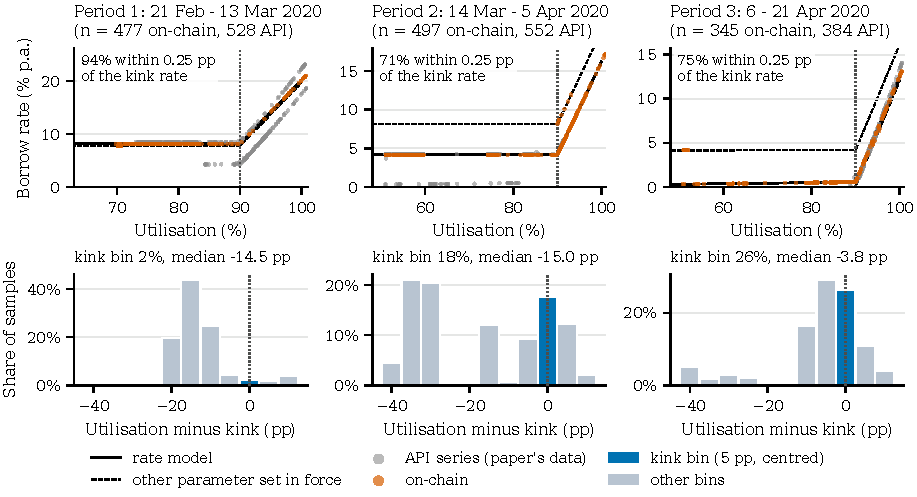
\includegraphics[width=\textwidth]{figures/report_fig1_kink.pdf}
\caption{Compound's DAI market in the paper's three kink periods, hourly. Top: borrow rate against utilisation; on-chain rates (orange), the API series the paper used (grey), and the rate model (solid: the parameter set in force for most of the period; dashed: other sets in force). The API reports compounded yields, the model simple rates. Bottom: utilisation minus kink in 5\pp\ bins; the bin centred on the kink is blue.}
\label{fig:kink}
\end{figure*}

% ======================================================================
\section{Construction of New Data}
\label{sec:newdata}

The paper's kink claim was tested on two datasets: one constructed from the blockchain and one existing dataset collected from its official source. A third, small dataset of governance texts was annotated. Figure~\ref{fig:snippet} shows extracts.

\subsection{Dataset 1: on-chain cDAI panel (constructed)}

\emph{Why.} The Compound API that supplied the paper's series is closed, its units were undocumented, and some periods disagree with the chain. The chain records the rates actually charged.

\emph{Collection.} We read the state of the cDAI contract and of its rate model from an archive node through \texttt{eth\_call} at fixed block intervals: every 6,000 blocks (about 20--22 hours) from 23 November 2019 to 30 November 2025, 2,489 samples, ending before Compound V2 was deprecated; and every 300 blocks (about one hour) from 21 February to 21 April 2020, 1,319 samples, covering the paper's three periods. Each sample records the borrow and supply rates, cash, borrows, reserves, the reserve factor, and the address and parameters of the model in force. The collector resumes after interruption, fails rather than saving incomplete data, and records its provenance without keys.

\emph{Preprocessing and annotation.} Block numbers were converted to timestamps by interpolating a sampled block-time table (median error 112 seconds); utilisation was computed with the contract's own formula. Each of the authors' 11 parameter regimes was labelled by rules committed before the script ran (matching on-chain change, source of the change, parameter agreement, reliability of the original series, number of liquidations).

Table~\ref{tab:regimes} shows the result. Regime~10 is matched by the pre-specified rule to the wrong change: the correct one, a new model contract, took effect 5.4 days after the authors' date, a flaw in the rule that we recorded in a post-hoc note without changing the labels. One on-chain change, a reserve-factor change in November 2019, has no regime in the authors' table. The original series is reliable (median gap to the chain $\le$0.25\pp) in only 4 of 11 regimes.

\begin{table}[t]
\centering\small
\setlength{\tabcolsep}{3pt}
\begin{tabular}{@{}rllrr@{}}
\toprule
Regime & On-chain timing & Parameters & API gap & Liq. \\
\midrule
0 & -- & RF differs & 0.94 & 20 \\
1 & +1.6 days & RF differs & 2.20 & 22 \\
2 & matches & match & 2.04 & 18 \\
3 & matches & match & \textbf{0.11} & 3 \\
4 & matches & match & 0.86 & 5 \\
5 & matches & match & 0.77 & 18 \\
6 & matches & match & 0.34 & 655 \\
7 & matches & match & \textbf{0.09} & 165 \\
8 & matches & match & \textbf{0.04} & 13 \\
9 & +0.5 days & match & 2.96 & 7 \\
10 & see text & multiplier differs & \textbf{0.22} & 21 \\
\bottomrule
\end{tabular}
\caption{Rule-based annotation of the authors' 11 DAI rate regimes against the chain. API gap: median absolute difference (pp) between the original series and on-chain rates; bold where reliable ($\le$0.25\pp). Liq.: liquidation events. RF: reserve factor, which does not enter the borrowing rate.}
\label{tab:regimes}
\end{table}

\emph{Quality checks.} Rates computed from the recorded parameters match the rates read from the contract to within 0.003\pp. The regime with most liquidations (655) contains the crash of 12 March 2020, as expected. A stratified random sample of 30 rows (from both panels and Dataset~2) was re-read from a second provider; the criterion was committed first, and all compared fields were identical in 30 of 30 rows.

\subsection{Dataset 2: Aave V3 (existing)}

To test whether the findings extend beyond Compound, we collected daily reserve data for USDC, USDT, DAI and WETH on the Aave V3 Ethereum Core market from Aave's official subgraph, 1 February 2023 to 30 November 2025: 4,123 of 4,136 possible asset-days. The 13 missing asset-days are all USDT observations before the first available midnight reserve snapshot (the earliest USDT state in the subgraph is from the evening of 13 February 2023), consistent with the on-chain Pool contract, which returned no USDT reserve at any of those 13 sampled blocks. The subgraph does not keep the history of rate-model parameters, so the kink at each sampled block was read from the chain. A pre-specified check compared subgraph utilisation with utilisation from on-chain balances every seventh day; in four reserve-periods it departed by 0.7--1.9\pp, above the threshold of 0.5\pp, and the decision for those periods used the on-chain values, as the rule required. The criterion, committed before the data were examined, divides each reserve's history into three periods (February--December 2023, 2024, January--November 2025): 12 reserve-periods. Because the four reserves are not independent, ``generalises'' requires clustering in at least 8 of 12 \emph{and} in at least two of three periods for at least three assets; 4 or fewer means ``does not generalise''; anything between is mixed evidence. We added the asset condition after a simulated scenario showed that eight successes concentrated in two assets would otherwise count as general.

\subsection{Annotation and agreement}

\emph{Rule-based labels} (regimes in Dataset 1) are deterministic, so agreement statistics are not informative; their quality rests on the checks above. \emph{Judgement labels} were produced twice.

\emph{Authors' assessment of fit.} The researcher coded the authors' comments on the 11 regimes as good fit, poor fit or not stated. GPT-5, through the ChatGPT web interface, given the same definitions but not the researcher's labels, agreed on 11 of 11 ($\kappa=1.00$, \citealp{cohen1960coefficient}). The task is easy and the web model cannot be pinned, so this shows only that the definitions were applied consistently.

\emph{Governance rationales for kink changes.} Market data show where utilisation lies relative to the kink; governance records show how the kink is meant to function. The kink of the four Aave reserves changed 19 times (16 governance actions after merging same-day changes). For each action we downloaded the forum post that first specifies the new value (in seven of the eight threads stored, with SHA-256 hashes) and labelled three properties defined in a committed codebook: the main reason given (\code{rationale}: \code{LIQUIDITY\_BUFFER}, \code{CAPITAL\_EFFICIENCY}, \code{RATE\_STABILITY}, \code{ALIGNMENT}, \code{OTHER} or \code{NOT\_STATED}), how the text frames the kink relative to utilisation (\code{kink\_framing}: a level utilisation settles at, \code{SETTLE\_AT}; a level it should stay below, \code{KEEP\_BELOW}; or only a parameter, \code{PARAMETER\_ONLY}), and whether the change is called temporary (\code{temporary}). As recommended for LLM evaluators \citep{samuylova2026judge}, each label records one property in a few defined categories, and the human labels were fixed before the model was run. The researcher labelled all units and committed the labels before a local open-weight model, Qwen2.5-7B-Instruct \citep{qwen2024qwen25} through Ollama (recorded digest, temperature 0, fixed seed), labelled them with the codebook as its prompt; the script refused to run until the researcher's labels were committed. Language models are increasingly used to annotate text \citep{gilardi2023chatgpt}; we used a locally hosted open-weight model as a second annotator, recording its weights and inference settings to support reproducibility, which a web interface does not allow \citep{spirling2023open,kim2024prometheus}.

Agreement was 12 of 16 for the reason ($\kappa=0.64$), 8 of 16 for the framing ($\kappa=0.21$) and 15 of 16 for temporary changes ($\kappa=0.85$). The model labelled 14 of 16 units \code{KEEP\_BELOW}, so most framing disagreements reflect its preference for one category (Appendix~\ref{app:conf}). Disagreements were resolved by the researcher, assisted by an AI assistant that drafted a decision from the codebook rules, the passages on the kink and the researcher's notes: the final label was the researcher's in 3 of 13, the model's in 5 and neither in 5. Only disagreements were reviewed, so shared errors remain possible.

\emph{How this relates to LLM-as-judge.} In LLM-as-judge evaluation a model scores the outputs of another system and its verdict is the measurement \citep{zheng2023judging}. Here the model does not judge; it applies the same codebook as the researcher, and its labels serve to measure whether the codebook can be applied consistently. The judging role, deciding the final label where the two disagree, stays with the researcher. Biases documented for LLM judges apply to annotators too, so we report agreement before arbitration and keep the model's raw outputs.

\begin{figure}[t]
\centering\small
\setlength{\tabcolsep}{3pt}
\begin{tabular}{@{}rlrrr@{}}
\multicolumn{5}{@{}l}{\textbf{(a)} \texttt{data/onchain/cdai\_panel.csv}, derived fields} \\
\toprule
Block & UTC & Util. & Borrow & Kink \\
\midrule
9,655,575 & 2020-03-12 08:04 & 87.9\% & 8.15\% & 90\% \\
12,547,575 & 2021-06-01 08:50 & 75.3\% & 3.77\% & 80\% \\
17,383,575 & 2023-06-01 04:25 & 55.7\% & 2.78\% & 80\% \\
22,609,575 & 2025-06-01 11:32 & 79.8\% & 3.99\% & 80\% \\
\bottomrule
\end{tabular}

\vspace{6pt}
\begin{tabularx}{\columnwidth}{@{}X@{}}
\textbf{(b)} Governance unit A10: USDT, kink 94\%\,$\rightarrow$\,92\%, effective 28 August 2025 (Chaos Labs, forum post 22279/17) \\
\midrule
\emph{``Following the recent inflow of \$1B in redeposits originating from Huobi, an event that has contributed to market stabilization, Chaos Labs recommends restoring the Optimal Utilization parameter to its standard target of 92\%.''} \\
\midrule
Final labels: \code{ALIGNMENT}; \code{SETTLE\_AT}; temporary \code{no} \\
\bottomrule
\end{tabularx}
\caption{Extracts from the new data. (a) The constructed cDAI panel stores raw contract integers; utilisation and annual borrow rates are derived with the contract's own formulas. (b) One of the 16 annotated governance units, with its labels.}
\label{fig:snippet}
\end{figure}

% ======================================================================
\section{Results on New Data}
\label{sec:results}

\paragraph{How the evaluation differs from the replication.} The paper judged clustering visually in three chosen periods. Our tests fix the periods (calendar years), the measure (the share of samples in the 5\pp\ bin centred on the kink, which must be the modal bin) and the decision rule before seeing the data, add a moving-block bootstrap for robustness \citep{kunsch1989jackknife}, and were checked on simulated data with known answers (81 of 81 and 180 of 180 decisions correct). For each dataset the criterion defines three verdicts: generalises, does not generalise, and mixed evidence.

\begin{table}[t]
\centering\small
\setlength{\tabcolsep}{3pt}
\begin{tabular}{@{}lrrr@{}}
\toprule
\textbf{cDAI} & Share & & \\
\midrule
\multicolumn{4}{@{}l}{\emph{Paper's periods (hourly)}} \\
21 Feb--13 Mar 2020 & 0.02 & & \\
14 Mar--5 Apr 2020 & 0.18 & & \\
6--21 Apr 2020 & 0.26 & & \\
\multicolumn{4}{@{}l}{\emph{New periods (daily)}} \\
May--Dec 2020 & \textbf{0.55} & & \\
2021 & \textbf{0.34}$^{r}$ & & \\
2022 & 0.02 & & \\
2023 & 0.21 & & \\
2024 & 0.23 & & \\
Jan--Nov 2025 & \textbf{0.34} & & \\
\midrule
\textbf{Aave V3} (daily) & 2023 & 2024 & 2025 \\
\midrule
USDC & \textbf{0.49} & \textbf{0.48} & 0.00$^{c}$ \\
USDT & \textbf{0.40} & \textbf{0.36} & 0.15$^{c}$ \\
DAI & \textbf{0.29} & \textbf{0.60}$^{c}$ & 0.02$^{c}$ \\
WETH & 0.09 & \textbf{0.33} & 0.28 \\
\bottomrule
\end{tabular}
\caption{Share of samples in the 5\pp\ bin centred on the kink; \textbf{bold} where that bin is the modal bin, i.e.\ clustering holds. $^{r}$Not robust (modal in 66\% of bootstrap resamples). $^{c}$Decided on weekly on-chain utilisation (subgraph failed its check). Clustering holds in 0 of 3 paper periods, 3 of 6 new cDAI periods and 7 of 12 Aave reserve-periods.}
\label{tab:newresults}
\end{table}

\begin{figure*}[t]
\centering
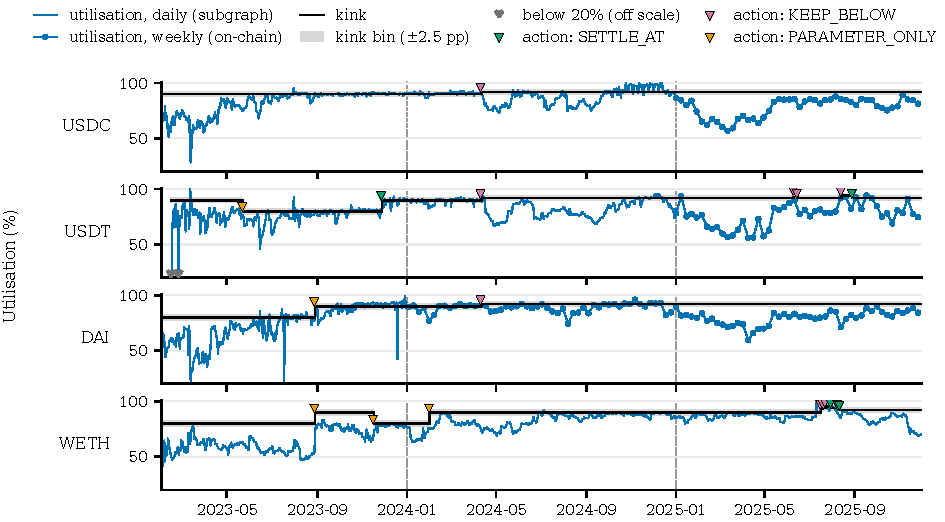
\includegraphics[width=\textwidth]{figures/report_fig_aave.pdf}
\caption{Aave V3 utilisation, kink and governance actions, February 2023 to November 2025. The shaded band is the test's kink bin (kink $\pm2.5$\pp); dashed lines separate the test's three periods. Triangles mark the 16 governance actions by framing, drawn just above the new kink for visibility. Lines with markers are weekly on-chain values where the subgraph failed its check; grey arrows mark values below the 20\% axis limit. A descriptive timeline, not an event study.}
\label{fig:aave}
\end{figure*}

\paragraph{Clustering.} Table~\ref{tab:newresults} gives the results. On cDAI, utilisation clusters at the kink in 3 of the 6 new periods, the pre-specified threshold for mixed evidence. One of the three, 2021, holds but not robustly: the kink bin is the modal bin, as the main rule requires, but it remains modal in only 66\% of 2,000 moving-block bootstrap resamples (14-day blocks), below the 80\% the criterion sets for a robust result. The criterion, committed in advance, counts a period that holds ``robustly or not'' towards the total; had 2021 been counted as not holding, the verdict would have been ``does not generalise'' (2 of 6) rather than mixed. On Aave V3, clustering holds in 7 of 12 reserve-periods, again mixed evidence; the distributions for cDAI are shown in Appendix~\ref{app:cdai}. The strongest case, cDAI in May--December 2020, largely overlaps with the COMP distribution, which from 15 June 2020 rewarded suppliers and borrowers in proportion to their balances \citep{wan2020comp}; it may have changed utilisation independently of the kink, and we do not separate the two. Clustering is observed alongside periods of elevated borrowing demand (cDAI in late 2020, the Aave stablecoins in 2023--2024), while periods of lower utilisation show less clustering: in 2025 median utilisation of the three stablecoins lay 10 to 14\pp\ below the kink in force, and their modal bins moved below it. WETH in 2025 is a near miss: 28\% of days fell in the kink bin, but the modal bin was the one just below. The analysis does not identify a causal effect of borrowing demand on clustering, and the 12 Aave periods are not independent.

\paragraph{How governance describes the kink.} These market patterns do not identify a mechanism; governance records add evidence on the kink's intended role. Table~\ref{tab:gov} gives the final labels. The six changes made through governance votes in 2023--2024 mostly changed the kink as a parameter, for capital efficiency. The ten changes made in 2025 by Aave's risk manager through the Risk Steward process treated the kink as a ceiling in periods of stress, raising it temporarily after large withdrawals to dampen rate spikes, and as a target when restoring it (``its standard target of 92\%''; ``our utilization target''). The second framing parallels the paper's Schelling-point reading in governance language, but is not evidence of coordination. It records intent, not outcome: how often utilisation lies near the target is what the clustering test measures, and there the evidence is mixed. Process and period coincide, so the difference between the groups cannot be attributed to the process. Figure~\ref{fig:aave} places the actions against utilisation and the kink: the 2025 changes came in short sequences, four on USDT between June and August and six on WETH between July and August.



\begin{table}[t]
\centering\small
\begin{tabular}{@{}lcc@{}}
\toprule
Final label & 2023--24 & 2025 \\
\midrule
\multicolumn{3}{@{}l}{\code{rationale}} \\
\quad\code{CAPITAL\_EFFICIENCY} & 4 & 1 \\
\quad\code{LIQUIDITY\_BUFFER} & 2 & 2 \\
\quad\code{RATE\_STABILITY} & 0 & 5 \\
\quad\code{ALIGNMENT} & 0 & 2 \\
\multicolumn{3}{@{}l}{\code{kink\_framing}} \\
\quad\code{PARAMETER\_ONLY} & 4 & 0 \\
\quad\code{SETTLE\_AT} & 1 & 4 \\
\quad\code{KEEP\_BELOW} & 1 & 6 \\
\multicolumn{3}{@{}l}{\code{temporary}} \\
\quad\code{yes} & 0 & 4 \\
\midrule
Actions & 6 & 10 \\
\bottomrule
\end{tabular}
\caption{Final labels of the 16 governance actions after arbitration: the six changes made through governance votes in 2023--24 and the ten made through the Risk Steward process in 2025. Codes as in the codebook; \code{OTHER} and \code{NOT\_STATED} were not used.}
\label{tab:gov}
\end{table}

\paragraph{Relation to the replication.} Neither dataset shows clustering of utilisation at the kink as a general feature of the markets and periods sampled; it occurs in some periods only, and not in the paper's. What the paper observed in rates is real, but it is a property of the model's shape, which governance can and does change.

\paragraph{Why the results differ from the paper.} Three differences in method separate our assessment from the paper's. First, the paper looked at rates, which a nearly flat model holds near the kink rate whatever utilisation does; we judged utilisation, the quantity a Schelling point concerns. Second, the paper used the API series, whose rates were compounded and whose utilisation departs from the chain by 3.6 to 11.2\pp\ in its three periods; we used on-chain values. Third, the paper chose three periods; we fixed calendar periods in advance. None of these makes the paper's figure wrong, but together they change what it can show.

\paragraph{Limitations.} The clustering measure is a single modal-bin rule applied to the distribution of utilisation within each period; it does not estimate how utilisation moves towards or away from the kink. When utilisation is centred on the kink but widely spread, simulations showed that it often returns ``does not hold'', so a negative verdict means that the kink is not the most common utilisation level, not that utilisation is unrelated to it. The periods within each dataset are not independent. The Aave sample covers four reserves of one market. The governance annotation has 16 units, a codebook written after the texts were read, and arbitration of disagreements only.

% ======================================================================
\section{Ethical Considerations}

\emph{Pseudonymous data.} The authors' event logs, redistributed in our repository because their code needs them, contain borrower and liquidator addresses. Addresses are pseudonymous, but they can be linked to identities through exchanges and other public information \citep{meiklejohn2013fistful}, and aggregating a person's activity increases this risk. The datasets we built contain only aggregates (rates, balances, counts per regime) and no account addresses; we did not attempt to identify any account. One governance post discusses withdrawals by a named exchange; we analysed only the published reasoning of the risk managers, who are public organisations writing in an official capacity.

\emph{Data minimisation and secondary use.} The new datasets record only contract-level state and model parameters, not transactions or accounts. Public availability does not make every use appropriate; aggregate analysis of public protocols is the use least likely to harm individuals.

\emph{AI annotators.} Model annotators can favour particular labels (here, one framing for 14 of 16 units), so we report agreement before arbitration, keep raw outputs, and do not assume model labels are right.

\emph{Licences and redistribution.} The original repository has no licence. Our repository is a GitHub fork of it, so the authors' code and data are reproduced under GitHub's terms for forks \citep{github2026terms}; we also asked the authors about redistribution on 27 October 2026 and had no reply by submission. Our licence covers only the files we wrote. Forum posts are stored in full only where they carry a CC0 waiver (19 of the 73 posts in the eight downloaded threads, including 13 of the 16 annotated); the others are replaced by their URL and the SHA-256 of their text, and a script downloads and verifies them, so the annotation can still be reproduced. We quote only short passages here. Raw price downloads remain subject to their providers' terms.

\emph{Research integrity.} Following the principles of honesty and transparency in the \citet{nhmrc2018code}, deviations and corrections are reported (Section~\ref{sec:replication}), and no keys or credentials are stored in the repository.

\emph{Use of AI.} Claude (Anthropic) and ChatGPT (OpenAI) were used to discuss the study design, to draft and debug analysis scripts, to review criteria and code, and to draft and edit this report, which the author revised; every number was checked against the committed outputs, and every source was read by the author. AI models also acted as annotators in two places, reported in Section~\ref{sec:newdata}, and an AI assistant drafted the arbitration decisions that the researcher reviewed.

% ======================================================================
\section{Conclusion and Reflections}

The paper's descriptive results and its cointegration model reproduce from the authors' code and data; its UIP coefficients do not, and the replacement of its exchange-rate source is likely to contribute to the difference. For the kink, the evidence forms a chain: rates near the kink rate reproduce (the phenomenon); on-chain, the model is almost flat below the kink and the original data mixed compounded and simple rates (the investigation); rates near the kink rate therefore cannot identify whether utilisation clusters at the kink (the inference); and a pre-specified utilisation test finds clustering in 0 of 3 of the paper's periods and in 3 of 6 and 7 of 12 new periods (the test). The phenomenon reproduces but does not suffice for its interpretation, and in the markets tested utilisation does not cluster at the kink as a general pattern under the pre-specified criterion. The two ``mixed'' verdicts differ in strength: on cDAI one of the three supporting periods is not robust, and without it the verdict would be ``does not generalise''; on Aave, 7 of 12 periods hold, one short of ``generalises''. The evidence is mixed, not a refutation.

Three reflections. First, the most consequential findings came from checking data, not code: API units and the shape of the rate model. Second, agreeing test decisions are weak evidence of reproduction when $p$-values are extreme or near a threshold; coefficients should be compared. Third, fixing criteria in advance exposed our own errors as well as the paper's: an assumption in our kink criterion that did not hold, a mistaken exchange-rate window, and categories in the annotation that a small model could not apply consistently. Each is reported rather than corrected silently, so that the limits of the findings can be audited.

With hindsight, we would fix the UIP criterion, coefficients included, before the first run; test the kink by rates and utilisation; and pilot the codebook with two annotators.

% ======================================================================
\bibliography{references}

\appendix
\sloppy
\raggedbottom
\renewcommand{\dbltopfraction}{0.85}
\renewcommand{\dblfloatpagefraction}{0.6}

\section{Reproduced Figures of the Paper's Section 5.1}
\label{app:repro}
The paper's Figures~1--5 are drawn by the authors' functions (\nolinkurl{scripts/reproduce_exploration.py}); its Figure~6 is redrawn from the authors' balances. Scripts for the other figures: \nolinkurl{scripts/make_appendix_figures.py} (appendix) and \nolinkurl{scripts/make_report_figures.py} (Figures~\ref{fig:kink} and~\ref{fig:aave}).

\begin{figure}[H]
\centering
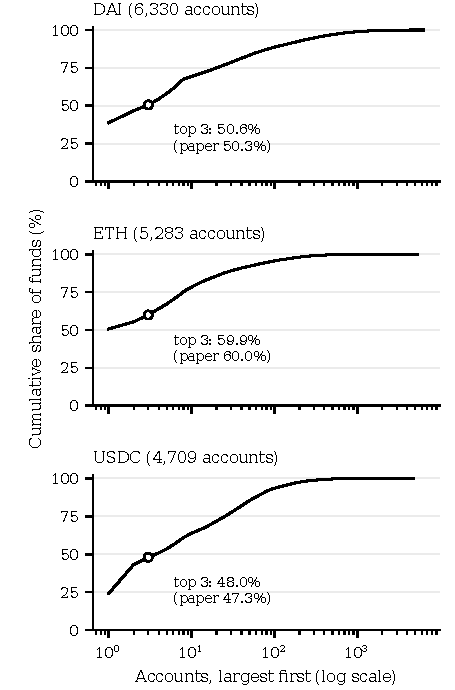
\includegraphics[width=\columnwidth]{figures/appx_concentration.pdf}
\caption{Paper's Figure~6, redrawn: cumulative share of funds by account on 4 June 2020. The three largest accounts hold 50.6, 59.9 and 48.0\% (paper: 50.3, 60.0, 47.3).}
\end{figure}

\begin{figure*}[!t]
\centering
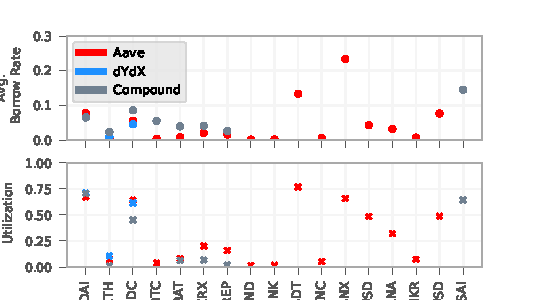
\includegraphics[width=0.58\textwidth]{figures/reproduction/platforms.pdf}
\caption{Paper's Figure~1: mean utilisation and borrow rate by token and protocol.}
\end{figure*}

\begin{figure*}[!t]
\centering
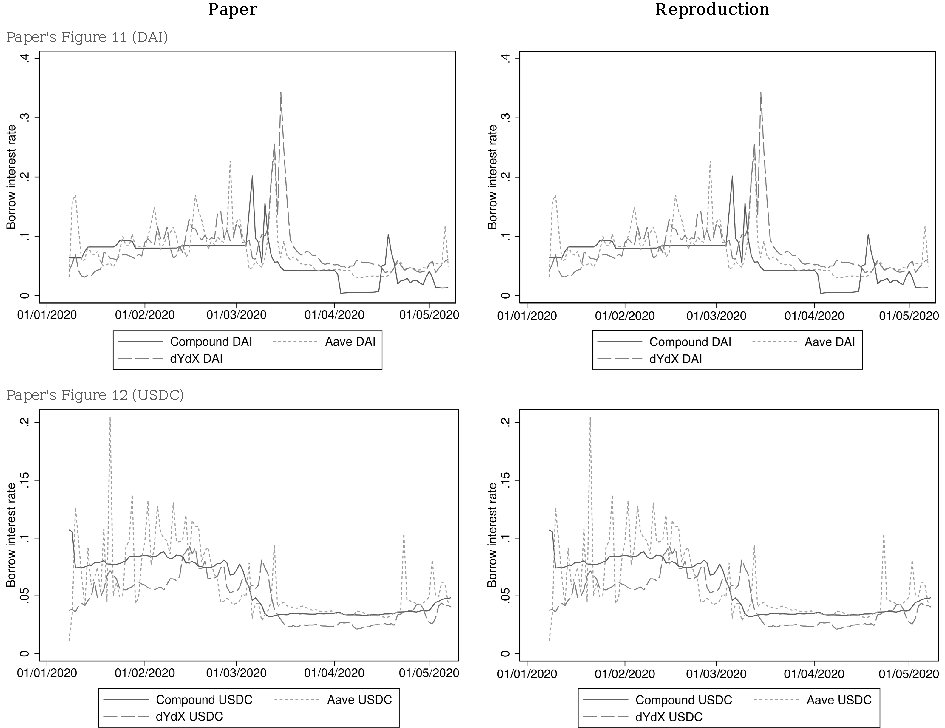
\includegraphics[width=\textwidth]{figures/appx_vecm_rates.pdf}
\caption{Borrow rates for DAI and USDC on the three protocols: the paper's Figures~11--12 and our reproduction, aligned on their axes (Appendix~\ref{app:vecm}).}
\label{fig:vecm}
\end{figure*}

\begin{figure*}[!t]
\centering
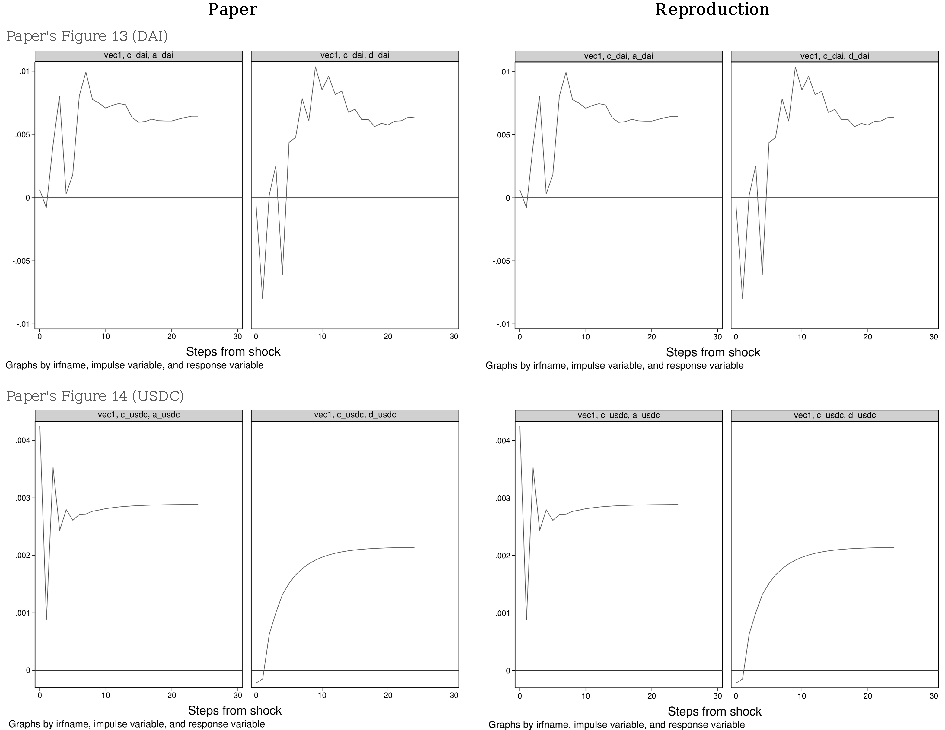
\includegraphics[width=\textwidth]{figures/appx_vecm_irf.pdf}
\caption{Impulse responses for DAI and USDC: the paper's Figures~13--14 and our reproduction, aligned on their axes (Appendix~\ref{app:vecm}).}
\label{fig:vecmirf}
\end{figure*}

\begin{figure}[H]
\centering
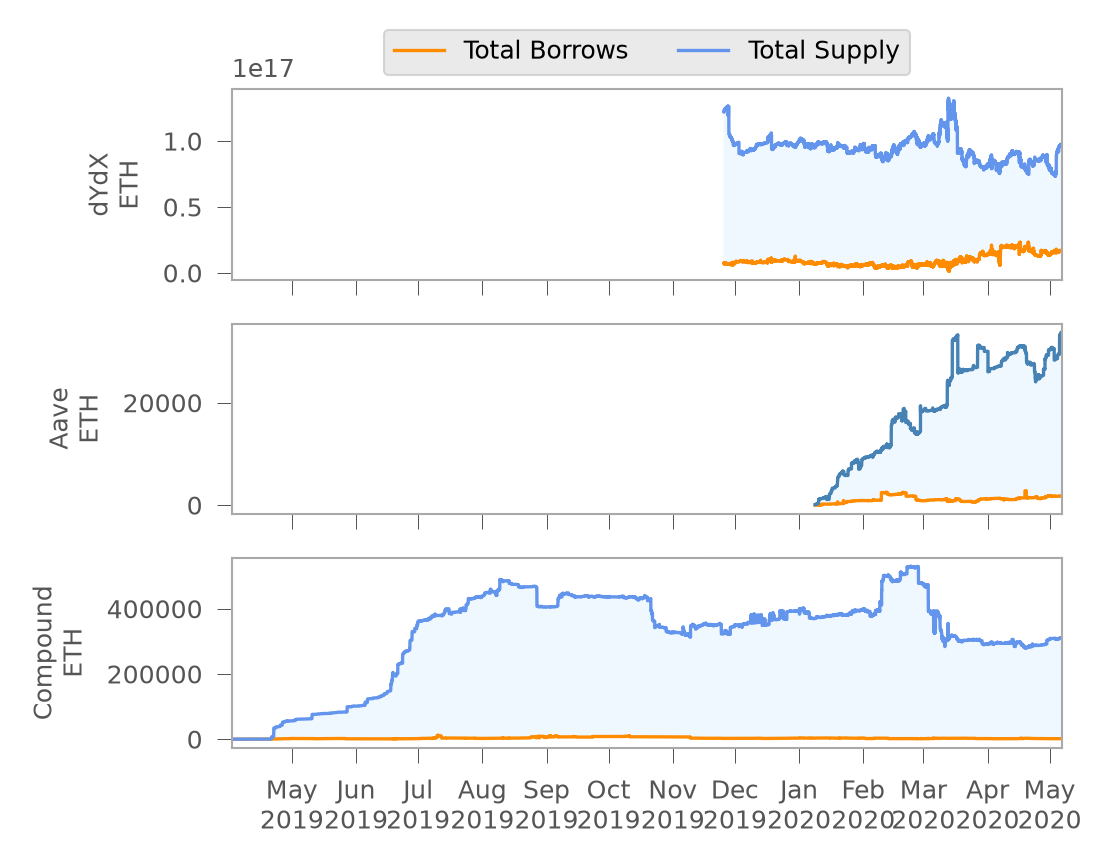
\includegraphics[width=\columnwidth]{figures/reproduction/eth-plf-liquidity.png}
\caption{Paper's Figure~2: ETH market liquidity, utilisation above 80 and 90\% shaded. The dYdX axis is off by $10^{12}$ (Section~\ref{sec:replication}).}
\end{figure}

\begin{figure}[!tp]
\centering
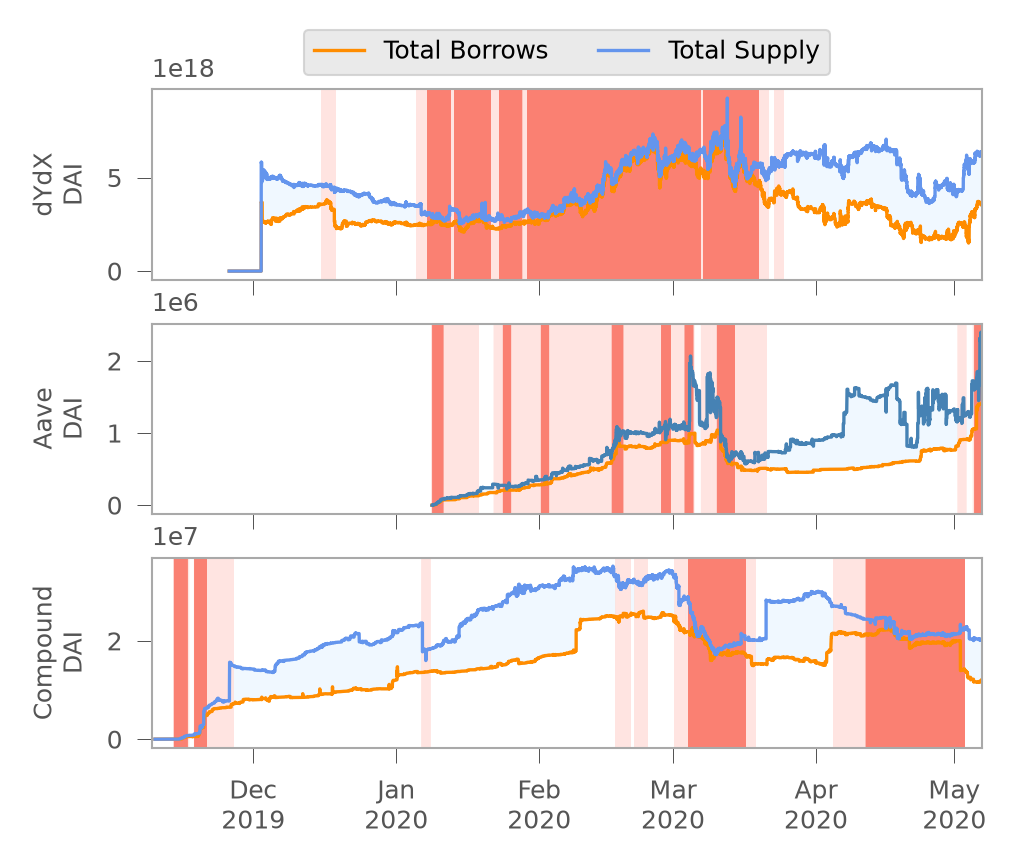
\includegraphics[width=\columnwidth]{figures/reproduction/dai-plf-liquidity.png}
\caption{Paper's Figure~3: DAI market liquidity.}
\end{figure}

\begin{figure}[!tp]
\centering
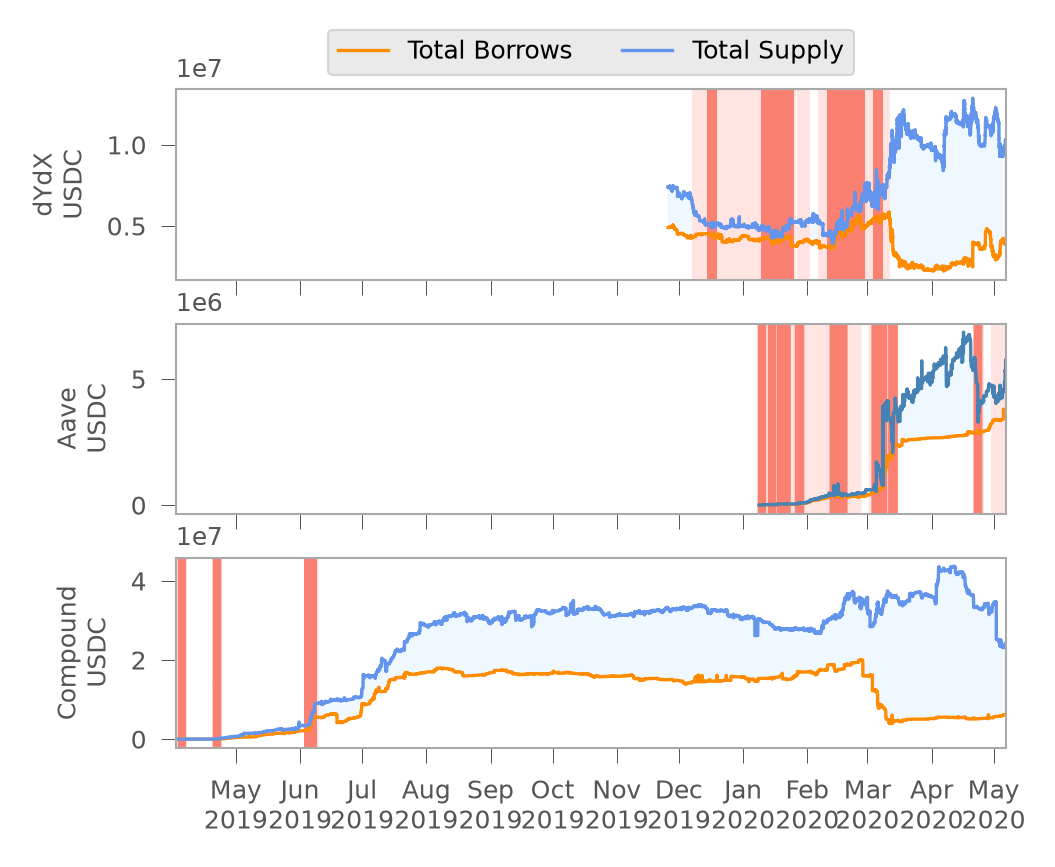
\includegraphics[width=\columnwidth]{figures/reproduction/usdc-plf-liquidity.png}
\caption{Paper's Figure~4: USDC market liquidity.}
\end{figure}

\begin{figure}[!tp]
\centering
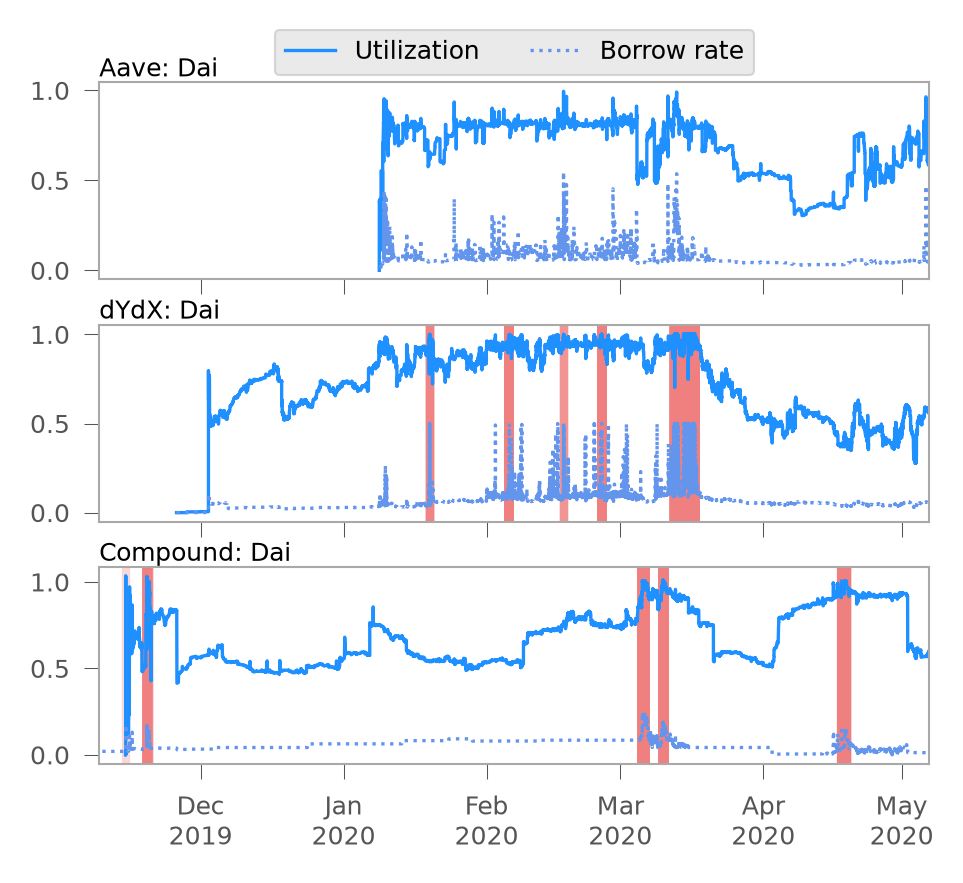
\includegraphics[width=\columnwidth]{figures/reproduction/dai-plfs-illiquidity.png}
\caption{Paper's Figure~5: DAI utilisation at or above 100\% (red), on Compound and dYdX but not Aave. The committed notebook calls this function only for USDC; we called it for DAI.}
\end{figure}



\section{VECM Figures: Paper and Reproduction}
\label{app:vecm}
Figures~\ref{fig:vecm} and~\ref{fig:vecmirf} set the paper's VECM figures, read as vector graphics from its arXiv version \citep{gudgeon2020defi}, beside the same figures from the authors' Stata do-file run on the authors' data (\nolinkurl{scripts/vecm_replication.do}). Panels are cropped and scaled so that their axes coincide; within each figure the plot areas' proportions differ by under 1\% (\nolinkurl{scripts/make_vecm_comparison.py}).

\needspace{0.4\textheight}
\section{API Series against the Chain}
\label{app:api}
The API that supplied the paper's rates reports compounded yields, while the rate model gives simple rates. To test whether units explain the API's disagreement with the chain, we compare each regime's median absolute gap twice: with the API rate as stored, and after converting it to a simple rate.

As stored, 7 of the 11 regimes exceed the 0.25\pp\ tolerance; after conversion, 6 do. Conversion removes the gap in the paper's first kink period (regime~6: from 0.34 to 0.004\pp) but leaves the largest gaps almost unchanged (regimes 1, 2 and 9, 2 to 3.3\pp).

Units therefore explain the disagreement in the period the paper analyses, but not elsewhere: the larger gaps have a cause that conversion does not remove. For this reason the analyses use rates read from the chain rather than a converted API series.

\begin{figure}[H]
\centering
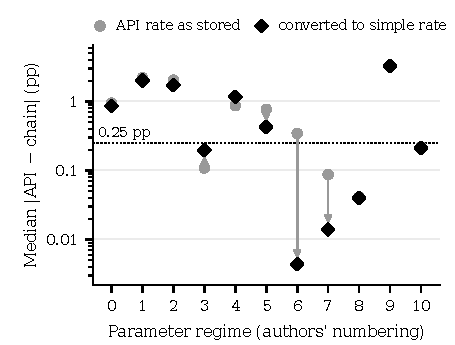
\includegraphics[width=\columnwidth]{figures/appx_api_gap.pdf}
\caption{Median gap between API and on-chain borrow rates, per regime. Dotted line: 0.25\pp\ tolerance. Regimes start at the authors' dates; Table~\ref{tab:regimes} starts each at its on-chain change, so regimes 1 and 9 differ slightly. Data: \nolinkurl{results/exploratory/apy_check.json}.}
\end{figure}

\needspace{0.42\textheight}
\section{Utilisation Relative to the Kink, New cDAI Periods}
\label{app:cdai}
\begin{figure}[H]
\centering
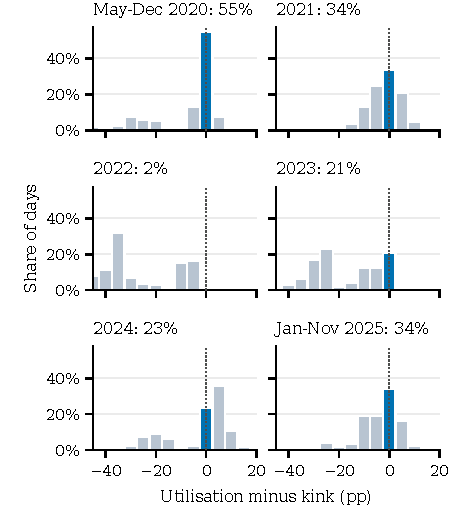
\includegraphics[width=\columnwidth]{figures/appx_cdai_periods.pdf}
\caption{Utilisation minus kink in the six new cDAI periods (daily; 5\pp\ bins, kink bin in blue). Days per period: 265, 392, 398, 434, 436, 398.}
\end{figure}

\needspace{0.52\textheight}
\section{Annotation Agreement before Arbitration}
\label{app:conf}
\begin{figure}[H]
\centering
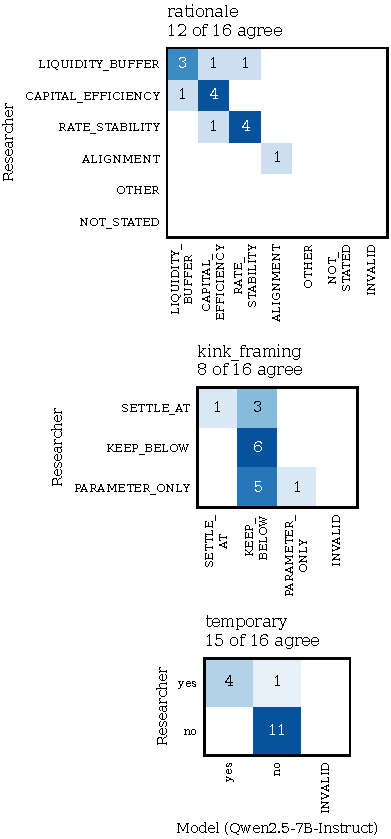
\includegraphics[width=\columnwidth]{figures/appx_confusion.pdf}
\caption{Researcher (rows) against model (columns) for the 16 units before arbitration; \code{INVALID} is output outside the codebook.}
\end{figure}

\end{document}
